\documentclass[12pt,a4paper]{report}
\usepackage[T1]{fontenc}
\usepackage[utf8]{inputenc}
\usepackage{mathpazo}
\usepackage[scaled=0.9]{helvet}
\usepackage{courier}
\usepackage{microtype}
\usepackage[a4paper,left=3cm,right=2.5cm,top=2.8cm,bottom=2.8cm]{geometry}
\usepackage{setspace}
\linespread{1.1}
\usepackage[table]{xcolor}
\definecolor{brand}{HTML}{24424D}
\usepackage{graphicx}
\usepackage{booktabs}
\usepackage{longtable}
\usepackage{array}
\usepackage{enumitem}
\usepackage{titlesec}
\usepackage{fancyhdr}
\usepackage{etoolbox}
\usepackage{needspace}
\usepackage{rotating}
\usepackage[font=small,labelfont=bf,labelsep=period,format=plain,skip=6pt]{caption}
\usepackage[hyphens,obeyspaces,spaces]{url}
\urlstyle{tt}
\renewcommand{\UrlFont}{\ttfamily\small}
\usepackage[colorlinks=true,linkcolor=brand,urlcolor=brand,citecolor=brand,pdftitle={Enterprise Resource Planning Data Platform (ERPDP)},pdfauthor={Ajith Abraham Ben, Kaviya V, Shaik Mohammad Shoyab}]{hyperref}

% ---- details shown on the title page. Leave a line empty to hide it.
\newcommand{\institution}{}
\newcommand{\guide}{}
\newcommand{\reportdate}{October 2026}

\newcommand{\code}[1]{\path{#1}}
\setlength{\parindent}{1.2em}
\setlength{\parskip}{0pt}
\setlist{itemsep=0.15em,topsep=0.4em,parsep=0pt}
\setlength{\LTpre}{6pt}\setlength{\LTpost}{6pt}
\setlength{\emergencystretch}{3em}
\renewcommand{\arraystretch}{1.15}

\titleformat{\chapter}[block]{\normalfont\huge\bfseries}{\thechapter\hspace{0.7em}}{0pt}{}[\vspace{3pt}\titlerule]
\titlespacing*{\chapter}{0pt}{-6pt}{26pt}
\titleformat{\section}{\normalfont\Large\bfseries}{\thesection\hspace{0.6em}}{0pt}{}
\titleformat{\subsection}{\normalfont\large\bfseries}{\thesubsection\hspace{0.6em}}{0pt}{}
\titleformat{\subsubsection}{\normalfont\normalsize\bfseries\itshape}{}{0pt}{}
\titlespacing*{\section}{0pt}{1.6em}{0.6em}
\titlespacing*{\subsection}{0pt}{1.3em}{0.45em}
\titlespacing*{\subsubsection}{0pt}{1em}{0.3em}

\pagestyle{fancy}\fancyhf{}
\renewcommand{\headrulewidth}{0.3pt}
\fancyhead[L]{\small\itshape\nouppercase{\leftmark}}
\fancyhead[R]{\small\thepage}
\renewcommand{\chaptermark}[1]{\markboth{\thechapter\hspace{0.5em}#1}{}}
\fancypagestyle{plain}{\fancyhf{}\renewcommand{\headrulewidth}{0pt}\fancyfoot[C]{\small\thepage}}

\newcommand{\tabsize}{\small}

\renewcommand{\bibname}{References}
\begin{document}

% ====================================================== title page
\begin{titlepage}
\centering
\ifdefempty{\institution}{\vspace*{1.2cm}}{{\Large\scshape\institution\par}\vspace{1.2cm}}
{\large\scshape Capstone Project Report\par}
\vspace{0.35cm}
{\color{brand}\rule{0.38\linewidth}{0.8pt}}\par
\vspace{1.9cm}
{\fontsize{27}{33}\selectfont\bfseries Enterprise Resource Planning\\[0.15cm] Data Platform (ERPDP)\par}
\vspace{0.8cm}
{\Large\itshape Design, implementation and validation of a data warehouse\\ for ten ERP datasets\par}
\vspace{2.0cm}
{\color{brand}\rule{0.38\linewidth}{0.8pt}}\par
\vspace{1.2cm}
{\normalsize Submitted by\par}
\vspace{0.4cm}
{\large Ajith Abraham Ben\par}
{\large Kaviya V\par}
{\large Shaik Mohammad Shoyab\par}
\ifdefempty{\guide}{}{\vspace{0.9cm}{\normalsize Under the guidance of\par}\vspace{0.3cm}{\large\guide\par}}
\vfill
{\normalsize M.Tech.\ Data Engineering\par}
\vspace{0.15cm}
{\normalsize Project UC15 \textperiodcentered{} Case organisation: ABC Global Enterprises Ltd.\par}
\vspace{0.15cm}
{\normalsize\reportdate\par}
\vspace{0.7cm}
{\small\color{brand}\href{https://github.com/7-Kaviya/Data-Engineering-UC15}{github.com/7-Kaviya/Data-Engineering-UC15}\par}
\end{titlepage}

% ====================================================== front matter
\pagenumbering{roman}
\setcounter{page}{1}

\chapter*{Abstract}
\addcontentsline{toc}{chapter}{Abstract}
\markboth{Abstract}{}
Organisations that run an ERP system usually keep finance, sales, procurement, inventory, manufacturing, personnel, warehouse, asset and customer data in separate modules, in different file formats and with different levels of quality. This project builds a data platform that brings ten such datasets into a single PostgreSQL data warehouse for a fictional company, ABC Global Enterprises Ltd. The data moves through raw, cleaned and warehouse layers. Pentaho Data Integration loads fifteen star-schema tables holding 78,558 rows, and one job runs the whole chain, from the raw files to a reconciled warehouse, in about seven seconds.

Row counts and control totals agree at every layer. Thirty-two automated checks on the finished warehouse give 21 passes and 11 known problems of the source data, and none of the results is unexpected. The work also produced a source-to-target mapping of all 141 warehouse columns, a metadata repository, a business glossary, lineage documentation, two real-time ingestion prototypes and two Tableau dashboards.

The most important result is a negative one. The ten datasets cannot be joined to each other, because customer, item and supplier identifiers differ from module to module and each module covers different years. We recorded twelve data quality findings of this kind and designed the warehouse as independent star schemas that share only a calendar dimension.

\bigskip\noindent\textbf{Keywords:} data warehouse, ETL, star schema, PostgreSQL, Pentaho, data quality, data lineage.

\clearpage
\tableofcontents
\clearpage
\listoffigures
\addcontentsline{toc}{chapter}{List of Figures}
\clearpage
\listoftables
\addcontentsline{toc}{chapter}{List of Tables}
\clearpage

\chapter*{List of Abbreviations}
\addcontentsline{toc}{chapter}{List of Abbreviations}
\markboth{List of Abbreviations}{}
\begin{tabular}{@{}p{2.6cm}p{11cm}@{}}
API & Application programming interface\\
BRD & Business Requirement Document\\
CSV & Comma-separated values\\
DDL & Data definition language\\
ERD & Entity relationship diagram\\
ERP & Enterprise resource planning\\
ETL & Extract, transform, load\\
JSON & JavaScript Object Notation\\
REST & Representational state transfer\\
SQL & Structured Query Language\\
XML & Extensible Markup Language\\
\end{tabular}

\clearpage
\pagenumbering{arabic}
\setcounter{page}{1}

% ====================================================== chapter 1
\chapter{Introduction}

\section{Background}
Most medium and large companies run their daily operations on an enterprise resource planning (ERP) system. The finance team posts its transactions in one module, the sales team in another, and procurement, inventory, manufacturing, warehouse management and human resources each have a module of their own. Every module stores data in whatever form suited its developers, so one exports CSV files, another XML and a third a relational dump. When management asks a question that crosses modules, for example how much was spent with suppliers in a month compared with what was sold, somebody has to collect the exports by hand and reconcile them in a spreadsheet. The answer arrives late, and nobody can say how far it can be trusted.

This project deals with that situation for a fictional company, ABC Global Enterprises Ltd., which is the case study of the capstone use case UC15. The company's ERP data is represented by ten datasets covering finance, sales, procurement, inventory, manufacturing, human resources, warehouse management, asset management, customer master data and accounts receivable. The task was to build an ERP Data Platform (ERPDP): a system that collects these datasets, cleans and validates them, stores them in a data warehouse and prepares them for reporting. A data warehouse in the sense of Inmon~\cite{inmon} is a subject-oriented, integrated, time-variant and non-volatile collection of data that supports decision making, and the platform was built to that description.

\section{Problem statement and objectives}
Three difficulties stand in the way of enterprise reporting at the company. The data is spread over modules with no common store. It arrives in several formats, namely CSV, Excel, JSON, XML and SQL. Nobody has measured its quality. The Business Requirement Document (BRD) turns these difficulties into seven objectives. The platform should:
\begin{enumerate}
\item collect business data from several ERP modules;
\item clean, validate and standardise transactional and master data;
\item store the curated data in a PostgreSQL data warehouse;
\item maintain metadata, audit logs and end-to-end data lineage;
\item support operational, analytical and financial reporting and executive dashboards;
\item use Git and GitHub for collaborative version control;
\item produce documentation and deliverables to enterprise standard.
\end{enumerate}

\section{Scope}
The work covers the ingestion of the ten datasets, their profiling, cleaning and validation, a star-schema warehouse in PostgreSQL, SQL reporting and dashboards. The BRD excludes real-time streaming, the replacement of the ERP system itself and mobile applications. Real-time ingestion was nevertheless explored during the second sprint, and after the sprint review a second prototype that reads a public REST interface was added at the request of the reviewing professor (Section~\ref{sec:realtime}). Neither prototype is part of the warehouse proper.

\section{Approach}
The project followed Agile Scrum in four sprints (Table~\ref{tab:sprints}). Every sprint ended with a review, and all code and documents were kept in one GitHub repository. At the time of writing the repository holds 70 commits from the three members of the team.

\begin{table}[htbp]
\centering\tabsize
\caption{The four sprints of the project.}\label{tab:sprints}
\begin{tabular}{@{}c p{3.6cm} p{8.4cm}@{}}
\toprule
Sprint & Focus & Main results\\
\midrule
0 & Initiation and architecture & Business Requirement Document, project charter, architecture, product backlog, repository structure\\
1 & Data discovery and ingestion & Source inventory, data dictionary, eleven ingestion transformations, PostgreSQL staging\\
2 & Profiling and the warehouse & Profiling, cleaning and validation, data quality report, star schema, warehouse load, reporting queries, reconciliation, real-time prototypes\\
3 & Governance, lineage and analytics & Load jobs with an audit log, source-to-target mapping, metadata, glossary, lineage, quality checks, dashboards\\
\bottomrule
\end{tabular}
\end{table}

\section{Organisation of this report}
Chapter~\ref{ch:data} describes the source data and the quality problems found in it, because these shaped the rest of the design. Chapter~\ref{ch:design} presents the architecture and the dimensional model. Chapter~\ref{ch:impl} describes how each part was built. Chapter~\ref{ch:results} reports the results of the reconciliation and the quality checks and summarises what the data shows. Chapter~\ref{ch:disc} discusses the problems met and the limits of the work, and Chapter~\ref{ch:concl} concludes with suggestions for further work.

% ====================================================== chapter 2
\chapter{Source Data and Data Quality}\label{ch:data}

\section{The ten datasets}
The ten datasets are listed in Table~\ref{tab:sources}. They come in four file formats, they range from 35 rows (Employee) to 45,839 rows (Account), and no customer, item or supplier identifier matches across them. The Warehouse file needs a special remark: every record appears twice, so that the raw file holds 6,408 rows but only 3,204 distinct ones. Cleaning removes the copies, and this is the only dataset that loses rows between the raw file and the warehouse. A separate combined file (\code{erp_cleaned_data.csv}, 6,600 rows) also exists in the repository. It is not one of the ten official datasets and is not loaded into the warehouse; Section~\ref{sec:findings} explains why.

\begin{table}[htbp]
\centering\tabsize\setlength{\tabcolsep}{4pt}
\caption{The ten source datasets, with the number of rows before and after cleaning.}\label{tab:sources}
\begin{tabular}{@{}l l l r r@{}}
\toprule
Dataset & Format & Raw file & Raw rows & Cleaned rows\\
\midrule
Sales & CSV & \code{Sales_data.csv} & 1,000 & 1,000\\
Customer Master & JSON & \code{Customer_Master.json} & 1,500 & 1,500\\
Asset & XML & \code{Asset_data.xml} & 1,245 & 1,245\\
Account (receivables) & Excel & \code{Account_data.xls} & 45,839 & 45,839\\
Procurement & CSV & \code{procurement_all.csv} & 1,300 & 1,300\\
Employee & Excel & \code{employee_data.xls} & 35 & 35\\
Finance & CSV & \code{Finance_data.csv} & 1,000 & 1,000\\
Inventory & JSON & \code{Inventory_data.json} & 1,000 & 1,000\\
Manufacturing & XML & \code{Manufacturing_data.xml} & 1,000 & 1,000\\
Warehouse & CSV & \code{warehouse.csv} & 6,408 & 3,204\\
\bottomrule
\end{tabular}
\end{table}

\section{Profiling}
Before any cleaning we profiled each dataset in two Jupyter notebooks, five datasets in each. For every dataset we recorded its size, the type of every column, missing values, duplicate rows, whether the supposed key was unique, the range of every date column and the distribution of the categorical columns. The results are written up in the Data Profiling Report that accompanies this report.

Most of what profiling showed was reassuring. Almost every column is complete, and keys are unique apart from the duplicated Warehouse file. A few observations turned out to matter later. The Sales file has a single empty value. The Manufacturing file has 258 empty cells, and these are not random: they are the actual start and end times of exactly the 129 jobs whose status is Failed, since a job that failed never started. In the Procurement file 330 of the 1,300 purchase orders are cancelled, and cancelled orders still carry a full cost. Finally, the datasets cover different periods. Accounts receivable documents date from 2011 to 2016, sales and procurement orders from 2023 and 2024, warehouse restocks from 2024, the manufacturing jobs lie within the single week of 18 to 25 March 2023, and the finance transactions run from 2025 into 2027.

\section{Data quality findings}\label{sec:findings}
Profiling and the validation scripts described in Section~\ref{sec:cleaning} together produced twelve findings, which are listed in Table~\ref{tab:findings} together with the way each was handled. The findings do not describe errors introduced by our pipeline; they are properties of the data as supplied. We decided early on to document them and not to correct them, because any correction of a business value would have meant inventing data.

\begingroup\tabsize\setlength{\tabcolsep}{4pt}
\begin{longtable}{@{}p{0.7cm}p{6.3cm}p{7.2cm}@{}}
\caption{The twelve data quality findings and how each was handled.}\label{tab:findings}\\
\toprule
\textbf{No.} & \textbf{Finding} & \textbf{Handling in the platform} \\
\midrule
\endfirsthead
\caption[]{\emph{continued}}\\
\toprule
\textbf{No.} & \textbf{Finding} & \textbf{Handling in the platform} \\
\midrule
\endhead
\bottomrule
\endfoot
\bottomrule
\endlastfoot
1 & Customer IDs are different in Sales, Customer Master and Account & No link between Sales, Customer Master and Receivables; customer IDs kept as plain columns \\
2 & Item IDs are different across Inventory, Warehouse, Procurement and Sales & Two separate item dimensions (Inventory and Warehouse) \\
3 & The dates of the modules are in different years & Modules are analysed one by one; the calendar spans 2011 to 2027 \\
4 & Supplier names change for the same supplier ID & The supplier dimension keeps the ID only; the name stays on the order \\
5 & Finance cannot be linked to Sales or Procurement & Finance is a standalone fact table \\
6 & 129 manufacturing jobs have no actual start and end & The empty actual start is exactly the Failed jobs; the column allows empty values \\
7 & Employee has no ID column & Employees get a generated key only \\
8 & The combined dataset is not the same as the official datasets & The combined file is excluded from the warehouse and used only for cross-checks \\
9 & Dates in the Account (Accounts Receivable) data are not logical & Kept and flagged; lateness figures are indicative only \\
10 & Smaller issues in Customer and Sales & Kept as given; one value may be empty \\
11 & Cancelled purchase orders carry a quarter of the procurement cost & Spend reports leave out cancelled orders \\
12 & The finance measures do not add up & Kept as given; one finance measure is never recomputed from another \\
\end{longtable}
\endgroup

Two groups of findings have the largest effect. The first concerns identifiers (Findings 1 and 2). Sales identifies customers with codes such as \code{CUST001}, the customer master uses numeric codes such as \code{5001}, and the receivables file uses ten-digit numbers. The identifiers are the same in the raw, staged and cleaned files, so the cleaning did not cause the mismatch; it is present in the source. A sale or an invoice therefore cannot be linked to a customer in the master file. We also tried the idea that the identifiers follow the row order, but could not confirm it, because the datasets share no other column, such as a name or a city, that would allow a comparison. Items behave in the same way: inventory items are coded \code{ITM_001}, warehouse items \code{ITM10000} and procurement items \code{P109}, and when we compared the 1,000 inventory items with the 3,204 warehouse items we found no common identifier. The second group concerns time (Finding 3). Because the modules cover different years, a comparison across modules is meaningful only where periods overlap, and for most pairs of modules they do not.

The combined file mentioned above is the subject of Finding 8. It looked attractive, because in it the keys did match across modules: all 859 customers in its sales section also occur in its customer section. We traced its origin and found that its scripts read a separate set of files from a personal download folder and not the official datasets. The team member who prepared it explained that the official datasets could not be combined, since some columns had the same name but different data types, so she had used synthetic datasets that combine properly. The one section we could compare directly, Procurement, was identical to the official file (1,300 rows against 1,300). Because the warehouse should represent the ten real datasets, we excluded the combined file and used it only for cross-checks.

% ====================================================== chapter 3
\chapter{System Design}\label{ch:design}

\section{Architecture}
The platform is organised in layers through which the data moves in one direction, from the raw files to the people who read reports (Figure~\ref{fig:layers}). The layering follows the pattern commonly called a medallion architecture. The raw layer holds the ten source files exactly as they were delivered and is never modified. The silver layer holds the cleaned and validated files, together with two reference tables, a calendar and a list of months, that are generated by a script because no source system supplies them. The gold layer is the PostgreSQL database \code{uc15_dw}, which contains the star-schema tables used for reporting. Reports, reconciliation queries, metadata views and dashboards form the final layer of use.

\begin{figure}[htbp]
\centering
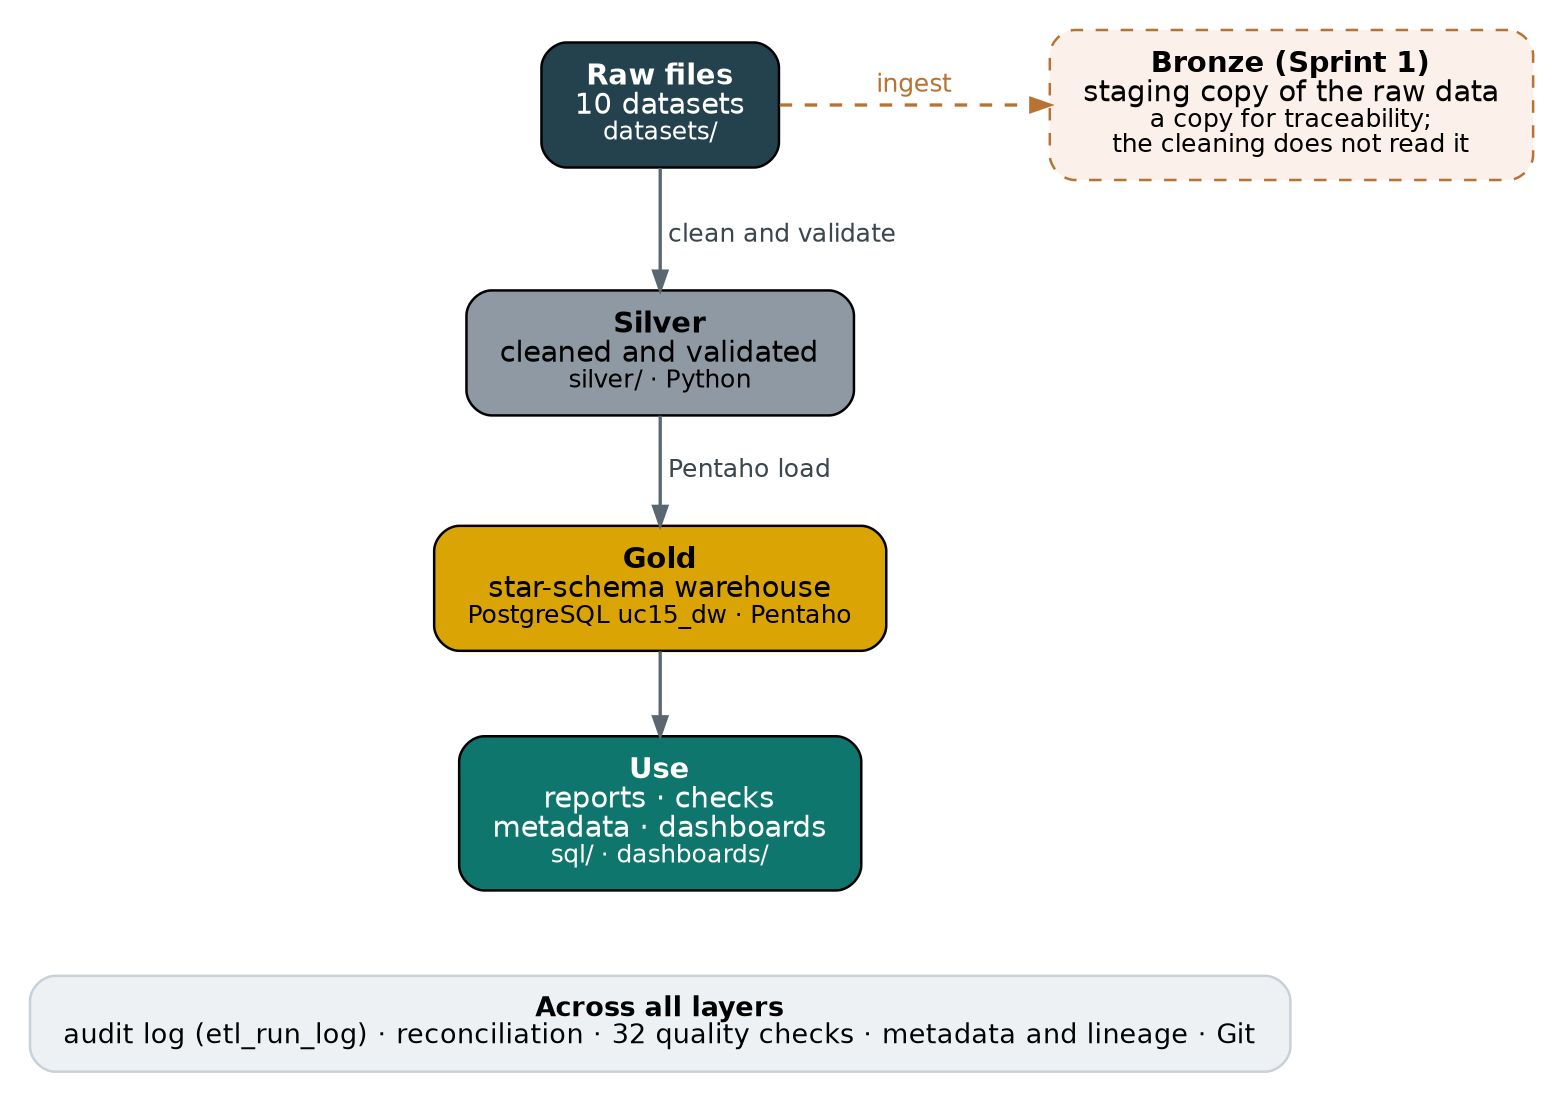
\includegraphics[width=0.78\textwidth]{figures/Architecture_Layers.png}
\caption{The layers of the platform. The bronze copy produced in the first sprint is kept for traceability; the cleaning scripts do not read it.}\label{fig:layers}
\end{figure}

A bronze layer also exists. In the first sprint each source file was loaded into a staging table in PostgreSQL by a Pentaho transformation, and a copy of every staging table was exported to the repository. In the finished platform the cleaning scripts read the raw files directly, so the bronze copy documents the ingestion but is not an input to the later layers. We return to this point in Section~\ref{sec:limits}.

\section{Technology}
Pentaho Data Integration 11.0 carries out the ingestion and the loading of the warehouse. It was chosen because the use case prescribes it and because its graphical transformations make the flow of each load visible. PostgreSQL 18 stores the warehouse and was inspected through pgAdmin. Python 3 with the pandas library is used wherever logic is easier to write as a script than as a transformation: profiling, cleaning, validation and the reconciliation of layers. Git and GitHub hold all code and documents. The Business Requirement Document names Power BI as the reporting tool; the dashboards were built in Tableau instead (Section~\ref{sec:dashboards}).

\section{The dimensional model}\label{sec:model}
For the design of the warehouse we followed the dimensional modelling approach described by Kimball and Ross~\cite{kimball}. The method starts from the questions that the business wants to answer, fixes the grain of each fact table, that is, what one row of it means, and only then decides which dimensions describe the facts. At each step we checked against the real data whether the links that the design assumed actually exist.

The check against the data decided the shape of the model. Since customer, item and supplier identifiers do not match across modules (Section~\ref{sec:findings}), a single connected star was not possible. The model therefore consists of seven fact tables, each with its own dimensions, joined to each other only through a shared calendar dimension, \code{DimDate}, which covers every day from 2011 to 2027. Table~\ref{tab:warehouse} lists the fifteen tables and Figure~\ref{fig:erd} shows how they are related.

\begingroup\tabsize\setlength{\tabcolsep}{4pt}
\begin{longtable}{@{}l l p{4.6cm} r r@{}}
\caption{The fifteen tables of the warehouse with their grain or content, number of rows and number of columns.}\label{tab:warehouse}\\
\toprule
\textbf{Table} & \textbf{Type} & \textbf{Content} & \textbf{Rows} & \textbf{Columns} \\
\midrule
\endfirsthead
\caption[]{\emph{continued}}\\
\toprule
\textbf{Table} & \textbf{Type} & \textbf{Content} & \textbf{Rows} & \textbf{Columns} \\
\midrule
\endhead
\bottomrule
\endfoot
\bottomrule
\endlastfoot
\code{DimMonth} & Dimension & The 12 months of the year, for seasonal demand. & 12 & 2 \\
\code{DimDate} & Dimension & Calendar of every day from 2011-01-01 to 2027-12-31. The only dimension shared by several facts. & 6,209 & 11 \\
\code{DimEmployee} & Dimension & Employees with salary, expenditure and savings. & 35 & 10 \\
\code{DimAsset} & Dimension & Equipment assets with condition, failures, maintenance cost and disposal decision. & 1,245 & 12 \\
\code{DimSupplier} & Dimension & Suppliers, identified by supplier ID only. & 10 & 2 \\
\code{DimCustomerMaster} & Dimension & Customers with contact details, address, type, status and credit limit. & 1,500 & 12 \\
\code{DimItemInventory} & Dimension & Items in the inventory module. & 1,000 & 5 \\
\code{DimWarehouseItem} & Dimension & Items in the warehouse module, with category and zone. & 3,204 & 5 \\
\code{FactSales} & Fact & Sales transactions. One row per transaction. & 1,000 & 11 \\
\code{FactFinance} & Fact & Finance transactions. One row per transaction. & 1,000 & 13 \\
\code{FactManufacturing} & Fact & Production jobs. One row per job. & 1,000 & 12 \\
\code{FactAccountsReceivable} & Fact & Accounts receivable documents. One row per document. & 45,839 & 14 \\
\code{FactProcurement} & Fact & Purchase orders. One row per order. & 1,300 & 12 \\
\code{FactWarehouseSnapshot} & Fact & Stock position of each warehouse item. One row per item. & 3,204 & 17 \\
\code{FactInventoryDemand} & Fact & Monthly demand of each inventory item. One row per item and month. & 12,000 & 3 \\
\textbf{Total} &  &  & \textbf{78,558} & \textbf{141} \\
\end{longtable}
\endgroup

\begin{figure}[htbp]
\centering
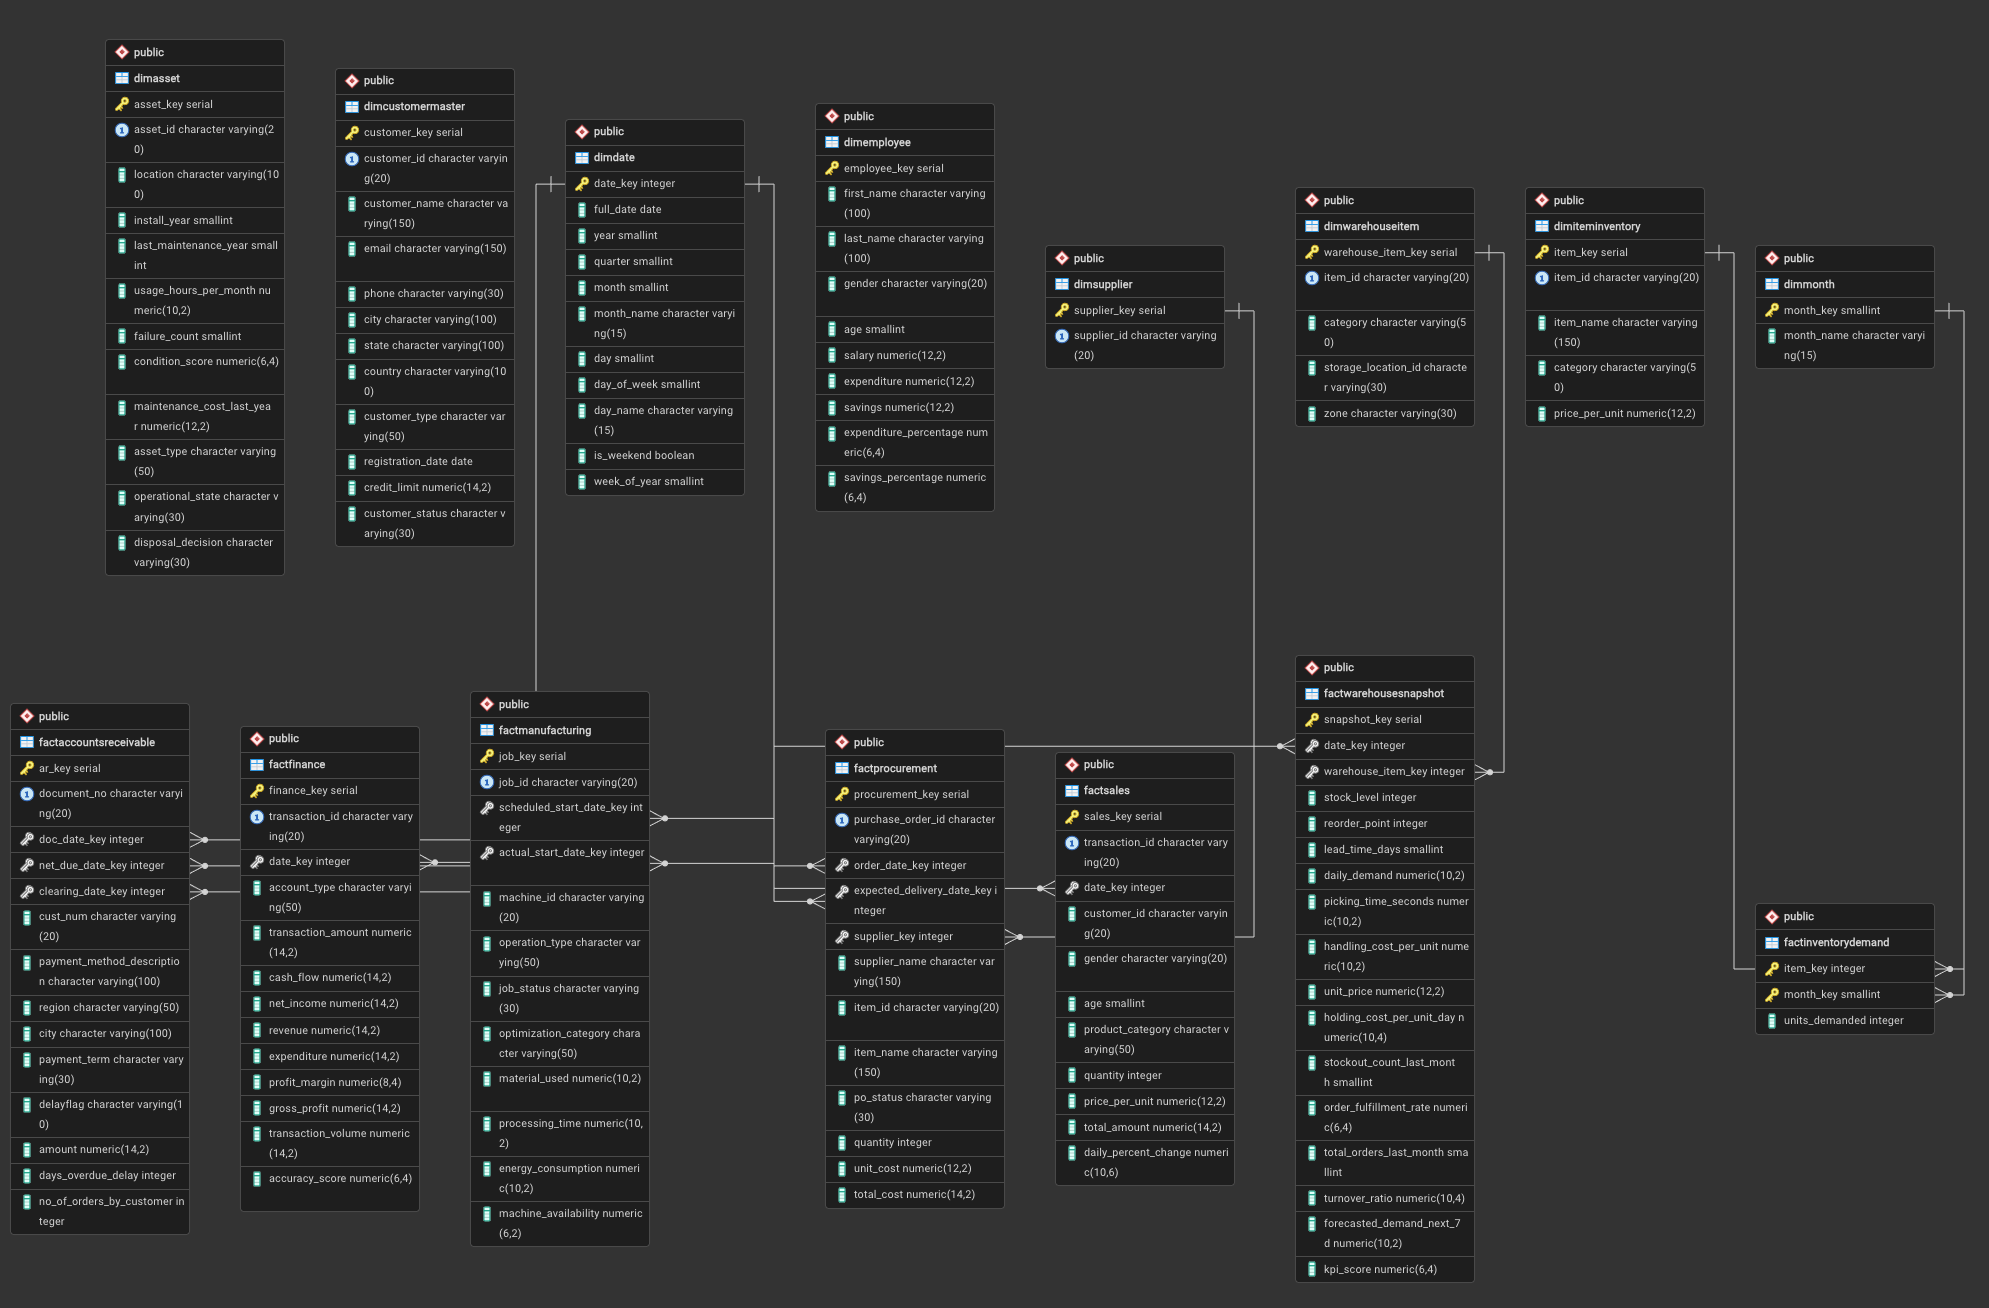
\includegraphics[width=\textwidth]{figures/ERD_uc15_dw.png}
\caption{Entity relationship diagram of the warehouse \texttt{uc15\_dw}, exported from pgAdmin.}\label{fig:erd}
\end{figure}

Several decisions in the model follow directly from the findings. Every dimension has a surrogate key generated by the database, so that the source identifiers, which are unreliable across modules, do not drive the design. The customer identifier in \code{FactSales} and the customer number in \code{FactAccountsReceivable} stay as ordinary columns, not foreign keys, because there is no dimension that they could point to. The supplier dimension holds the supplier identifier only, since the same supplier appears under several names (Finding 4), and the name stays with the order. The employee file has no identifier at all, so \code{DimEmployee} has only its surrogate key. The actual start date of a manufacturing job may be empty, because a failed job never started (Finding 6). Finally, the inventory file holds twelve demand columns, one per month and without a year, and it is stored as one row per item and month, which is why \code{FactInventoryDemand} has 12,000 rows for 1,000 items and uses a separate month dimension instead of the calendar.

\section{Load strategy and control}
The warehouse is loaded completely on every run. Every table is emptied and refilled, which is simple, safe for data of this size and easy to verify. Each load is compared with control totals, namely the row count and one numeric total per table, which are calculated independently from the cleaned files. All Pentaho transformations use paths relative to their own location and read the database password from a variable, so that no password is stored in the repository and the project runs unchanged on another computer.

% ====================================================== chapter 4
\chapter{Implementation}\label{ch:impl}

\section{Ingestion}
In the first sprint we recorded for each dataset its format, size and fields in a source inventory and a data dictionary. We then built eleven Pentaho ingestion transformations, one for each dataset and one for the combined file. They read CSV, Excel, JSON, XML and SQL sources, write them with only minor changes into staging tables, and log load errors. The Procurement and Warehouse transformations read the SQL versions of those datasets through a table input step. These transformations contain fixed paths of the machine on which they were built, which is acceptable for a staging exercise but means they cannot be rerun elsewhere without editing.

\section{Cleaning and validation}\label{sec:cleaning}
Two Python scripts, each responsible for five datasets, apply the same steps. They standardise column names to lower case with underscores, trim text, replace null-like strings by real nulls, convert dates to the form \code{YYYY-MM-DD} and numbers to numeric types, and remove blank rows and exact duplicate rows. In the customer file the nested contact and address records are kept as JSON text and are split into columns later by Pentaho. The sales dates arrive as day-month-year and are converted. Across all ten datasets the only rows removed are the 3,204 duplicate rows of the Warehouse file.

Two further scripts validate the cleaned files with 81 checks: 32 for the first group of datasets and 49 for the second. They test for missing values, duplicate keys, impossible values such as negative amounts or ages outside 18 to 100, unparseable dates and inconsistent totals. Seventy-six checks pass and five fail. All five failures describe real properties of the data and not defects of the pipeline: the 258 empty manufacturing cells, one empty sales value, customers with a registration date in the future (a count that falls as time passes), and receivable documents whose due date (11,269) or clearing date (12,104) precedes the document date.

\section{Loading the warehouse}
Fifteen Pentaho transformations, one per table, load the warehouse. They fall into four groups. The first loads dimensions that need no transformation beyond renaming columns. The second handles the calendar and month tables, which come from reference files written by a Python script, the supplier dimension, which keeps each supplier identifier once, and the customer dimension, where the JSON text is split into e-mail address, phone number, city, state and country. The third group loads facts that carry dates. Each date is converted to a text of the form \code{yyyyMMdd} and then to an integer, which is the key of \code{DimDate}. The fourth group loads facts that must find their dimension keys first: procurement looks up the supplier key, the warehouse snapshot looks up the item key, and the inventory demand transformation first turns the twelve monthly columns into twelve rows per item with a row normaliser step and then looks up the item key. Dimensions are loaded before facts. A Python loader that produces the same tables served as an independent cross-check during development.

\section{Orchestration and the audit trail}
Two Pentaho jobs tie the transformations together. The job \code{ETL_Load_Warehouse} writes a start entry to an audit table, resets all fifteen tables, loads the eight dimensions and then the seven facts, records the row count of every table, and finally runs the reconciliation against the control totals. If any step fails, or if one table does not match its control totals, the job writes a failure entry and aborts. The audit table, \code{etl_run_log}, stores a run identifier, the job and step names, a status and a message with a timestamp for every stage of every run.

The second job, \code{ETL_End_To_End}, starts one step earlier. It runs the two cleaning scripts and the two validation scripts, calls the load job, runs the script that compares all layers (Section~\ref{sec:recon}) and ends with a quality gate that stops the job if any of the checks of Section~\ref{sec:qchecks} returns an unexpected result. On the project laptop the whole chain, from the raw files to a reconciled warehouse, takes about seven seconds. We tested both ways in which the job can fail. A script that exits with an error stopped the job and was logged. A second test changed the quantity of one sale after loading. The row totals did not change, so the reconciliation passed, but the business rule that a total equals quantity times price was broken, and the quality gate caught it. This is the reason for having both kinds of control. The job needs Python on the search path of Pentaho's graphical tool, which is achieved by starting it from a terminal window.

\section{SQL reporting}
The file \code{sql/04_enterprise_reporting_queries.sql} contains 23 queries that exercise the warehouse as an analyst would. They cover sales by month, category, age band and the largest orders; procurement by supplier, month, item and status; inventory demand by category, season and item; warehouse stock, stockouts and zones; finance by account type and month; receivables ageing; manufacturing by machine, job status, energy and material; and one comparison of sales and procurement by month for 2023, the only year in which the two modules overlap. All queries were run against the loaded data.

\section{Real-time ingestion}\label{sec:realtime}
The BRD excludes real-time streaming, but two small prototypes were built to show how it would work. In the first, a producer script writes simulated sales events into a queue table and announces each of them with the \code{NOTIFY} mechanism of PostgreSQL~\cite{pgdocs}. A consumer script listens for the notification, validates the event (a positive quantity, a known product category, a date that exists in \code{DimDate}) and writes valid events to a real-time fact table. Events reached the fact table within one to six milliseconds, invalid events were rejected with a stated reason, and events that arrived while the consumer was stopped were waiting in the queue when it returned.

The second prototype uses a real external source, which the professor asked for after the sprint review. A script polls the public Coinbase price interface every five seconds for Bitcoin and Ethereum, validates each reading and stores it, with the response time of the request, in a separate database. A run of about sixteen and a half minutes stored 346 readings with a mean response time of 382 milliseconds, the slowest request taking 3,717 milliseconds, and no problem was logged. A set of nine queries derives the change since the first reading, one-minute candles with opening, high, low and closing price, a five-reading moving average, volatility and the largest jumps. The data also shows why such feeds need validation and smoothing: in one stretch the Bitcoin price alternated between two values 35.22 apart within about eleven seconds, which is more likely a difference between the servers answering than a real movement. Neither prototype is part of the warehouse.

\section{Metadata, glossary and lineage}\label{sec:lineage}
Governance was the theme of the third sprint. A source-to-target mapping workbook traces each of the 141 warehouse columns back to its raw file and column, its cleaned file and column, and the Pentaho rule that loads it. A metadata repository describes every table and column in plain language and lists the values and ranges observed in the data; the same descriptions are stored inside PostgreSQL as object comments, so that pgAdmin shows them and two views list them with SQL. A glossary defines 79 business and data terms. The lineage document draws the route of every dataset from its raw file to the reports that read it (Appendix~\ref{app:lineage}), traces three columns end to end, and states which tables and queries must be rerun when a source changes.

Writing the lineage document exposed three differences between the first sprint and the later work. The cleaning reads the raw files, not the bronze copy. The source inventory lists procurement as an SQL file with 2,000 rows dated 2026, whereas the warehouse is built from a CSV file of 1,300 rows dated 2023 and 2024. And the inventory lists the employee file with 1,500 rows and the receivables file with 45,856, whereas the files hold 35 and 45,839. None of these affects the correctness of the warehouse, but they should be settled with the team that prepared the sources.

\section{Dashboards}\label{sec:dashboards}
Eleven flat views, one for each dashboard area, join every fact table to its dimensions, so that a dashboard tool needs no knowledge of the star schema. They leave out the names, e-mail addresses and phone numbers of customers and employees, and they are exported to CSV files. The totals of every view equal the control totals of the warehouse, and every view has as many rows as its fact table. A nine-page dashboard design defines the measures and the figures that each page should show.

Two dashboards with ten sheets were built in Tableau from the exported files: sales by category, warehouse demand, receivable delay, procurement cost, finance revenue, machine availability, inventory demand by month, salary by age group, credit limit by city, and asset condition. Opened in Tableau Reader, the sales sheet adds up to 456,000, which is the sales total of the warehouse, and the values we compared on the demand and credit-limit sheets agree with it. The dashboards are simpler than the design. They carry no explanatory text and no page for data trust, and three sheets need correction: the procurement cost includes cancelled orders, the asset condition score is added up when an average is meant, and the delay days and the finance revenue appear without a warning that they are unreliable (Findings 9 and 12). A Power BI version was prepared as an alternative, with measures and a build guide, but was not built.

% ====================================================== chapter 5
\chapter{Results and Evaluation}\label{ch:results}

\section{Reconciliation from raw file to warehouse}\label{sec:recon}
The first question to ask of a data pipeline is whether it loses or invents anything. To answer it for every dataset we compare three layers, the raw file, the cleaned file and the warehouse, by the number of rows and by one control total. The total is the sum of the amount in sales, procurement, receivables and finance, the credit limit for customers, the salary for employees, the maintenance cost for assets, the material used in manufacturing, the stock level in the warehouse, and the sum of the twelve monthly demand columns for inventory. Table~\ref{tab:recon} shows the result.

\begingroup\tabsize\setlength{\tabcolsep}{4pt}
\begin{longtable}{@{}l r r r l@{}}
\caption{Row counts of the ten datasets in the raw file, the cleaned file and the warehouse.}\label{tab:recon}\\
\toprule
\textbf{Dataset} & \textbf{Raw rows} & \textbf{Cleaned rows} & \textbf{Loaded rows} & \textbf{Result} \\
\midrule
\endfirsthead
\caption[]{\emph{continued}}\\
\toprule
\textbf{Dataset} & \textbf{Raw rows} & \textbf{Cleaned rows} & \textbf{Loaded rows} & \textbf{Result} \\
\midrule
\endhead
\bottomrule
\endfoot
\bottomrule
\endlastfoot
Sales & 1,000 & 1,000 & 1,000 & identical \\
Customer Master & 1,500 & 1,500 & 1,500 & identical \\
Asset & 1,245 & 1,245 & 1,245 & identical \\
Account & 45,839 & 45,839 & 45,839 & identical \\
Procurement & 1,300 & 1,300 & 1,300 & identical \\
Employee & 35 & 35 & 35 & identical \\
Finance & 1,000 & 1,000 & 1,000 & identical \\
Inventory & 1,000 & 1,000 & 1,000 & identical \\
Manufacturing & 1,000 & 1,000 & 1,000 & identical \\
Warehouse & 6,408 & 3,204 & 3,204 & explained \\
\end{longtable}
\endgroup

Nine of the ten datasets have identical row counts and totals at all three layers. The Warehouse dataset differs between the raw and the cleaned file, and the difference is explained: the raw file holds every record twice, so its total (1,688,454) is exactly double that of the cleaned file and the warehouse (844,227), and cleaning removed 3,204 duplicate rows. In addition to this comparison, the warehouse itself is checked after every load against control totals calculated from the cleaned files. All fifteen tables match, for example the total of \code{FactSales} is 456,000.00 and that of \code{FactProcurement} is 982,390,348.71.

\section{Automated data quality checks}\label{sec:qchecks}
Matching totals show that data was moved correctly; they do not show that the data obeys the rules of the business. For this we wrote 32 checks in SQL as a single view on the finished warehouse. They fall into three groups (Table~\ref{tab:checkgroups}). Eleven integrity checks test that no foreign key points to a missing row, in one check covering all fourteen relationships, and that the business key of each of ten tables is unique. Ten business-rule checks test statements that should hold in any consistent dataset, for example that the total of a sale equals quantity times price, that an employee's salary equals expenditure plus savings, that a manufacturing job without an actual start date is a failed job, and that quantities and amounts are positive. Eleven further checks count the known problems of the source data and compare each count with the number documented in the Data Quality Report.

\begingroup\tabsize\setlength{\tabcolsep}{4pt}
\begin{longtable}{@{}p{6.4cm}r r r r@{}}
\caption{The 32 data quality checks by group and result.}\label{tab:checkgroups}\\
\toprule
\textbf{Group} & \textbf{Checks} & \textbf{Pass} & \textbf{Known issue} & \textbf{Unexpected} \\
\midrule
\endfirsthead
\caption[]{\emph{continued}}\\
\toprule
\textbf{Group} & \textbf{Checks} & \textbf{Pass} & \textbf{Known issue} & \textbf{Unexpected} \\
\midrule
\endhead
\bottomrule
\endfoot
\bottomrule
\endlastfoot
Integrity (keys and relationships) & 11 & 11 & 0 & 0 \\
Business rules & 10 & 10 & 0 & 0 \\
Known problems of the source data & 11 & 0 & 11 & 0 \\
\textbf{All checks} & \textbf{32} & \textbf{21} & \textbf{11} & \textbf{0} \\
\end{longtable}
\endgroup

Every check receives one of three statuses. A check passes if no row breaks the rule. It is a known issue if the rule is broken in exactly the way the Data Quality Report documents. It is unexpected if rows break the rule but their number differs from the documented count. The current result is 21 passes, 11 known issues and no unexpected result. The known issues are listed in Table~\ref{tab:known}. They quantify Findings 4, 9, 10, 11 and 12 on the finished warehouse: the contradictions between the receivable dates and the delay columns, the finance figures that do not follow accounting formulas, the cancelled orders, and the suppliers that appear under several names.

\begingroup\tabsize\setlength{\tabcolsep}{4pt}
\begin{longtable}{@{}l p{8.2cm} r l@{}}
\caption{The eleven known issues of the source data, as counted on the warehouse.}\label{tab:known}\\
\toprule
\textbf{Check} & \textbf{What is counted} & \textbf{Found} & \textbf{Finding} \\
\midrule
\endfirsthead
\caption[]{\emph{continued}}\\
\toprule
\textbf{Check} & \textbf{What is counted} & \textbf{Found} & \textbf{Finding} \\
\midrule
\endhead
\bottomrule
\endfoot
\bottomrule
\endlastfoot
K01 & Receivables: due date before the document date & 11,269 & Finding 9 \\
K02 & Receivables: clearing date before the document date & 12,104 & Finding 9 \\
K03 & Receivables: days\_overdue\_delay differs from clearing date minus due date & 16,910 & Finding 9 \\
K04 & Receivables: delayflag disagrees with days\_overdue\_delay above 0 & 5,797 & Finding 9 \\
K05 & Finance: net\_income differs from revenue - expenditure & 1,000 & Finding 12 \\
K06 & Finance: gross\_profit differs from revenue - expenditure & 1,000 & Finding 12 \\
K07 & Finance: profit\_margin differs from net\_income / revenue & 998 & Finding 12 \\
K08 & Customers registered after today (changes with the date) & 42 & Finding 10 \\
K09 & Sales: empty daily\_percent\_change & 1 & Finding 10 \\
K10 & Procurement: orders with status Cancelled & 330 & Finding 11 \\
K11 & Procurement: suppliers that appear under more than one name & 10 & Finding 4 \\
\end{longtable}
\endgroup

A check is only useful if it can fail, so we tested this. We changed one sales total and one delay flag inside a database transaction, observed that the two affected checks turned to the status unexpected, and rolled the transaction back. One remark about use: on an empty warehouse every check reports a pass, since there is nothing to break, so the checks are meaningful only after a load. The check for customers registered in the future depends on the current date and therefore has no fixed expected count.

\section{Reproducibility}\label{sec:repro}
The end-to-end job runs the cleaning scripts again on every execution, so it was necessary to know whether they reproduce the files stored in the repository. We ran both scripts on a clean copy and compared all ten cleaned files with the committed ones. Nine were identical byte for byte. The Finance file differed in the sixteenth or seventeenth significant digit of 22 numbers, a difference in floating-point formatting between versions of the software, not in the data.

The test also found a real problem. The date conversion of the second cleaning script was written to apply only to columns whose type is \code{object}. In version 3 of pandas~\cite{pandasdocs}, text columns have a new type, so the condition was never true, the conversion was skipped silently, and the 1,000 sales dates stayed in the form \code{24-11-2023}, which the Pentaho load cannot read. No error message appeared. The repair was two lines that treat both types as text. Afterwards all 1,000 sales dates were compared with the raw file read as day-month-year, including the 414 whose day is 12 or less and which could therefore be confused with a month, and every one was correct.

As a last test of reproducibility we rebuilt the whole warehouse from the files on GitHub alone, in a new database. It contained 78,558 rows, all fifteen control totals matched, the quality checks again gave 21 passes and 11 known issues, and all twelve exported dashboard files were identical to the committed ones.

\section{What the data shows}
Within the limits discussed below, the warehouse already answers useful questions, and the answers are the first reward of the pipeline. Sales are spread fairly evenly over three product categories, Electronics (156,905), Clothing (155,580) and Beauty (143,515), and female customers account for 51.1\% of the revenue. A quarter of the ordered procurement value, 25.1\% or 330 of 1,300 orders, was cancelled; without the cancelled orders the spend is about 735 million and the largest supplier, SUP004, accounts for 92.7 million of it. Of the receivable documents 65.7\% are flagged as delayed, but 30.5\% have dates that contradict each other, so the lateness is indicative only; half of the amount, 50.0\%, is paid by one payment method, Direct Debits 2.

Grocery makes up 84.5\% of inventory demand, and demand hardly changes during the year, March being only 1.2\% above August. In the warehouse 237 of 3,204 items (7.4\%) are below their reorder point and Zone D had the most stockouts in the last month (3,812). In manufacturing, 12.9\% of the jobs failed, and two machines fail more often than the other three: M04 with 17.6\% and M03 with 15.6\%, against 10.0\% to 10.9\%. Of the 1,245 assets, 67.6\% are obsolete, and recycling is the most common planned disposal (493 assets). Tamil Nadu has the most customers (379, or 25.3\%), and 92.9\% of all customers are active. The datasets are synthetic and the modules cover different years, so each of these findings stands alone and describes the data we have, not a real company.

% ====================================================== chapter 6
\chapter{Discussion}\label{ch:disc}

\section{Problems met during the project}
Some of the difficulties were technical. At one point the password of the local PostgreSQL superuser was lost. We recovered it by switching the access configuration file to trust mode for a short time, setting a new password, restoring password authentication and recreating the connection in pgAdmin. Early scripts and transformations contained absolute Windows paths of one team member's computer and failed on the others. The final load transformations and scripts use relative paths and a password variable instead. The pandas change described in Section~\ref{sec:repro} shows how a library update can alter results without raising an error, and the detection came from a test that ran the pipeline a second time and compared the result. A smaller surprise was that the graphical Pentaho tool prints the warnings that Python writes to its error stream in red as \textsf{ERROR}, even though the job succeeds.

The largest difficulty was not technical. It was the discovery that the datasets do not connect. We lost time looking for a join key that does not exist, and the combined file was a detour that ended with the decision to document the gap and not to hide it.

\section{Limitations}\label{sec:limits}
The work has the following limits.
\begin{itemize}
\item The modules cannot be combined. Questions that cross modules, such as the profit per customer, cannot be answered with this data, because customer, item and supplier identifiers and the years differ.
\item Some measures are unreliable. The receivable delay columns and the finance measures do not follow their usual formulas, and about a third of the finance transactions are dated after the date of this report.
\item The Tableau dashboards are simpler than the dashboard design and need the corrections described in Section~\ref{sec:dashboards}.
\item The bronze copy is not an input to the cleaning, and the source inventory of the first sprint differs from the files in three places (Section~\ref{sec:lineage}).
\item The warehouse is reloaded completely on every run. This suits the present data volume but would not suit a much larger system.
\item The data is synthetic, so conclusions about the business are illustrations.
\end{itemize}

% ====================================================== chapter 7
\chapter{Conclusion and Future Work}\label{ch:concl}
The project set out to build a data platform for ten ERP datasets, and it did so. The data is collected, cleaned, validated and loaded into a PostgreSQL star-schema warehouse by a single repeatable job that writes an audit log, and the result is checked at every layer: row counts and totals agree from the raw file to the warehouse, and 32 automated checks find nothing that is not already documented. Around the warehouse sit a source-to-target mapping, a metadata repository, a glossary, lineage documentation, SQL reports, two real-time prototypes and two Tableau dashboards.

The more instructive result is the documentation of what the data cannot do. The ten datasets do not join, several measures contradict their own definitions, and these facts are recorded in twelve findings and monitored by the checks, not corrected. A warehouse that reports these limits openly is more useful than one that conceals them.

Several things would improve the work. The Tableau dashboards should be brought closer to the design: cancelled orders left out of the cost, the condition score averaged, warnings added where figures are unreliable, and a page that shows the data trust. The team should agree on one official procurement dataset, correct the source inventory and rebuild the bronze layer from the files that the later layers use. If master data were available that links customers, items and suppliers across modules, the independent star schemas could be joined and the cross-module questions could finally be answered. The load could move from a complete reload to incremental loading, run on a schedule and alert someone on failure. The finance transactions that are dated after the report should be recorded as a thirteenth finding and covered by a check.

% ====================================================== references
\begin{thebibliography}{9}
\bibitem{kimball} R.~Kimball and M.~Ross, \emph{The Data Warehouse Toolkit: The Definitive Guide to Dimensional Modeling}, 3rd ed. Hoboken, NJ: Wiley, 2013.
\bibitem{inmon} W.~H.~Inmon, \emph{Building the Data Warehouse}, 4th ed. Hoboken, NJ: Wiley, 2005.
\bibitem{pgdocs} PostgreSQL Global Development Group, \emph{PostgreSQL Documentation}. Available: \url{https://www.postgresql.org/docs/}
\bibitem{pandasdocs} The pandas development team, \emph{pandas Documentation}. Available: \url{https://pandas.pydata.org/docs/}
\end{thebibliography}
\addcontentsline{toc}{chapter}{References}

% ====================================================== appendices
\appendix
\chapter{Deliverables by Sprint}\label{app:deliver}
Table~\ref{tab:deliver} lists the deliverables of the project and where each can be found in the repository.

\begingroup\tabsize\setlength{\tabcolsep}{4pt}
\begin{longtable}{@{}c p{5.9cm} p{7.4cm}@{}}
\caption{Deliverables of the project and their location in the repository.}\label{tab:deliver}\\
\toprule
\textbf{Sprint} & \textbf{Deliverable} & \textbf{Location} \\
\midrule
\endfirsthead
\caption[]{\emph{continued}}\\
\toprule
\textbf{Sprint} & \textbf{Deliverable} & \textbf{Location} \\
\midrule
\endhead
\bottomrule
\endfoot
\bottomrule
\endlastfoot
0 & BRD, charter, architecture, product backlog & \code{docs/} \\
1 & Source inventory and data dictionary & \code{docs/Source_Inventory.xlsx}, \code{bronze/ingestion/} \\
1 & 11 ingestion transformations and staging copies & \code{pentaho/transformations/}, \code{bronze/staging/} \\
2 & Data Profiling Report and notebooks & \code{docs/Data_Profiling_Report.md}, \code{python/} \\
2 & Cleaning and validation scripts and results & \code{python/}, \code{silver/} \\
2 & Data Quality Report (12 findings) & \code{docs/Data_Quality_Report.md} \\
2 & Star schema, warehouse and 15 load transformations & \code{sql/01_create_star_schema.sql}, \code{pentaho/transformations/} \\
2 & Reporting queries and reconciliation & \code{sql/04_enterprise_reporting_queries.sql}, \code{sql/05_reconciliation_checks.sql} \\
2 & Real-time ingestion (two versions) & \code{realtime_rest_demo/}, \code{python/realtime_*.py}, \code{sql/06_*}, \code{sql/07_*} \\
3 & Load job, end-to-end job and audit log & \code{pentaho/jobs/}, \code{sql/08_etl_audit_setup.sql} \\
3 & Source-to-target mapping, metadata, glossary & \code{metadata/}, \code{sql/09_metadata_comments.sql} \\
3 & Data lineage document and diagram & \code{lineage/} \\
3 & Validation Report, layer reconciliation and checks & \code{docs/Validation_Report.md}, \code{python/ERP_Layer_Reconciliation.py}, \code{sql/10_data_quality_checks.sql} \\
3 & Dashboard views, exported data, design and Tableau dashboards & \code{sql/11_dashboard_views.sql}, \code{dashboards/} \\
3 & README with how to run & \code{README.md} \\
\end{longtable}
\endgroup

\chapter{Data Lineage Diagram}\label{app:lineage}
Figure~\ref{fig:lineage} shows the route of every dataset from its raw file, through the cleaned file, to its warehouse tables and the consumers that read them. The dashed box at the top is the bronze copy of the first sprint, which is not read by the cleaning scripts.

\begin{sidewaysfigure}[p]
\centering
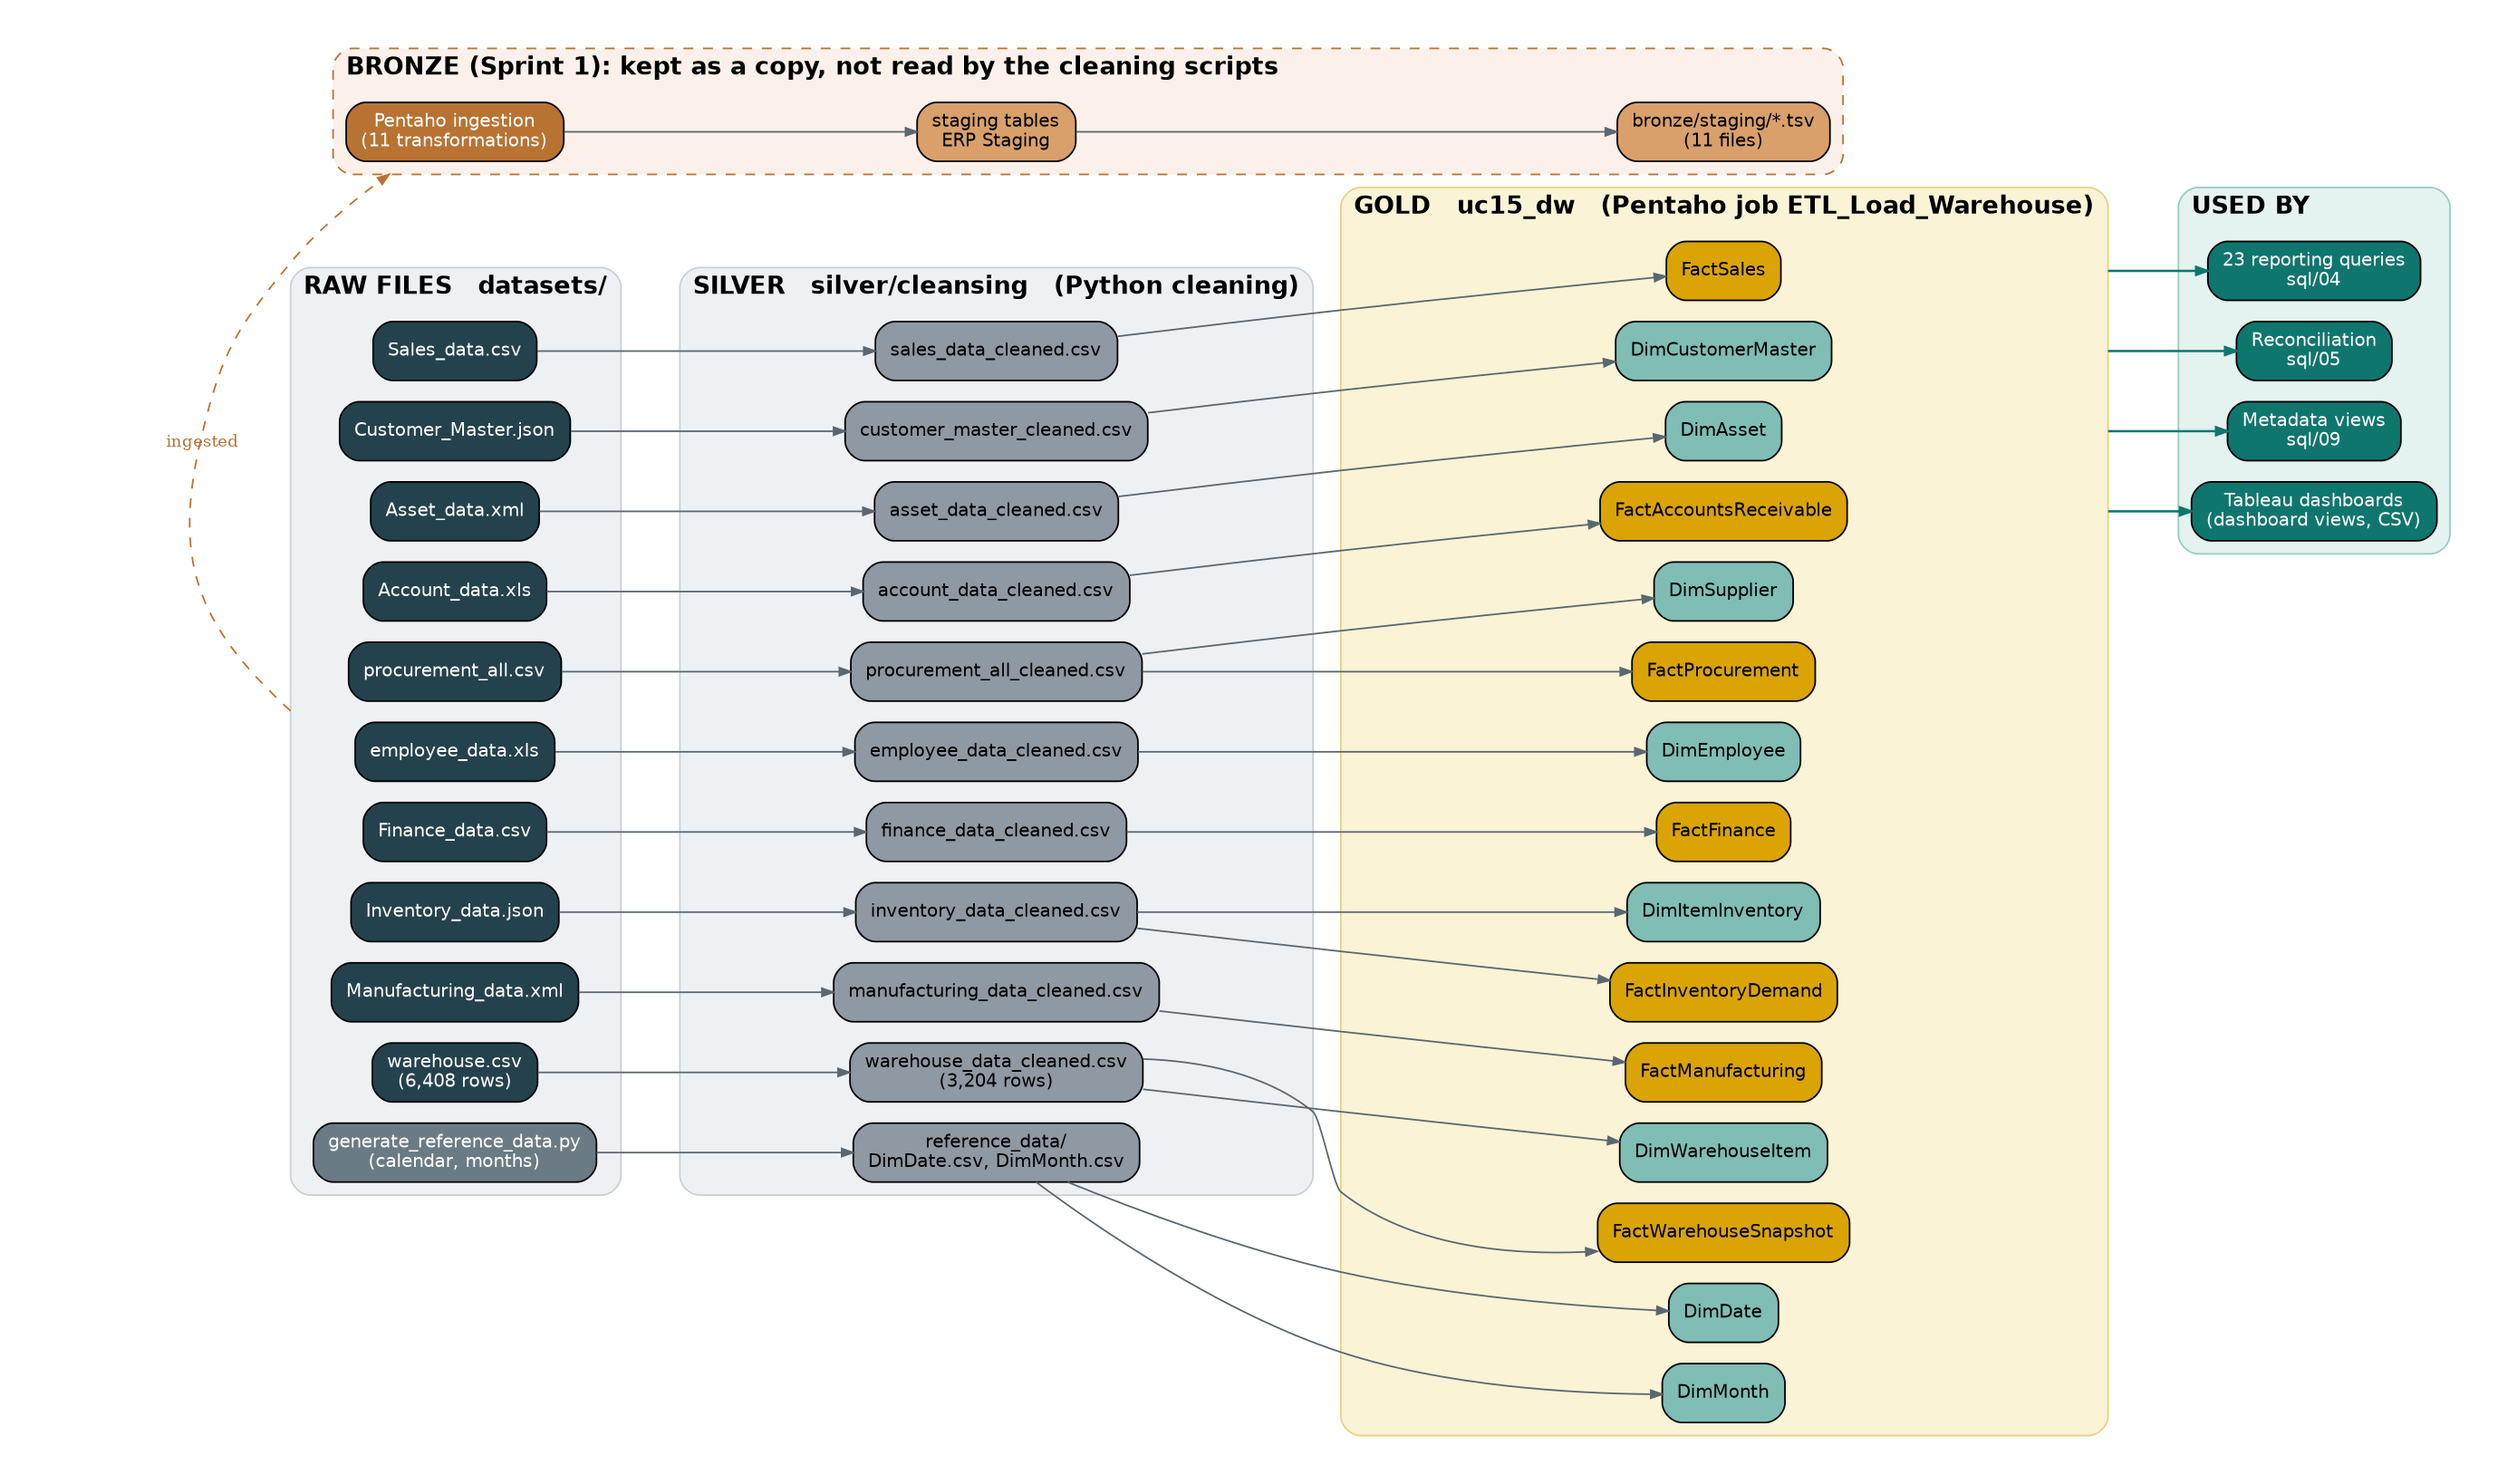
\includegraphics[width=22cm,height=12.4cm,keepaspectratio]{figures/Lineage_Diagram.png}
\caption{Data lineage of the ten datasets and the two reference tables.}\label{fig:lineage}
\end{sidewaysfigure}

\end{document}

